\documentclass{article}
\usepackage[utf8]{inputenc}
\usepackage{graphicx}
\title{Evaluacion 1}
\author{Roberto Alexis Gomez Pintor}
\begin{document}
\maketitle
\section{Introduccion}
La evaluacion se realizara con datos obtenidos Análisis de las mareas y salinidad en el Manglar El Sargento, en una bahía en la costa frente a la parte norte de la Isla
Tiburón.
\subsection{Manglar}
El manglar es un área biótica o bioma, formado por árboles muy tolerantes a las sales existentes en la zona intermareal cercana a la desembocadura de cursos de agua dulce en latitudes tropicales y subtropicales.
\subsection{Isla tiburon}
La isla Tiburón o isla del Tiburón. es una isla mexicana, la más grande del golfo de
California y tiene una extensión de 1208 km cuadrados. Administrativamente, pertenece al estado de Sonora, específicamente al municipio de Hermosillo, y se ubica aproximadamente a la misma latitud que Hermosillo. Está separada del continente por un estrecho canal de sólo tres kilómetros de ancho llamado estrecho del Infiernillo.
\section{Reporte.}
La evaluacion se realizo con los datos Análisis de las mareas y salinidad en el Manglar El Sargento. Al leer los 2 archivos observe que poco mas de 2100 renglones y 10 columnas de informacion sobre mareas y salinidad de solo el mes de Febrero del año en curso(2018) contenia, tambien lei las intrucciones de la pagina que resultaron algo engañosas: "\textbf{Usa los comandos de Linux y Emacs}", entendi que tenia que modificar los archivos, asi que estaba quitando fechas e informacion durante 1 hora. Hasta que se explico que no era necesario la modificacion de los archivos. Despues de eso se comenzo a trabajar con pandas en Jupyter Notebook, mediante ayuda de otros codigos y del profesor se colo los datos tanto el archivo de salinidad como el del nivel del agua. En el proceso se realizaron partes para obtener graficas tanto de salinidad, temperatura, nivel del agua y tiempo para su usos.
\section{Codigos}
Los siguientes condigos se utilizaron en Jupyter Notebook como principales para el desarrollo de la actividad. Se obtuvieron graficas de salinidad,temperatura y nivel del agua medidos contra el tiempo. Otras 2 graficas de comparacion de nivel del agua contra temperatura y salinidad.
\begin{verbatim}
import pandas as pd
import numpy as np
from datetime import datetime
\end{verbatim}
\begin{verbatim}
# Leer archivo de datos
# Convertir las columnas Temp, de objeto a número
df = pd.read_csv("sargento-2702181.csv", header=None,skiprows=2, names=['#','DateTime','AbsPres','Temp','WaterLevel'])
#df.DateTime=pd.to_numeric(df.DateTime, errors='coerce')
df.AbsPres=pd.to_numeric(df.AbsPres, errors='coerce')
df.head()
\end{verbatim}
\begin{verbatim}
# Leer archivo de datos
# Convertir las columnas Temp, de objeto a número
df1 = pd.read_csv("sargento-salinidad-2702181.csv", header=None,skiprows=2, names=['#','DateTime','CordonHigh','Temp','SpecificConductance','Salinity'])
#df.DateTime=pd.to_numeric(df1.DateTime, errors='coerce')
#df1.CondHigh=pd.to_numeric(df1.CondHigh, errors='coerce')
df1.head()
\end{verbatim}
\section{Graficas}
\subsection{Tiempo y Salinidad}
\begin{figure}[ht]
  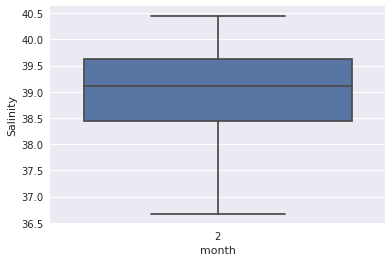
\includegraphics[width=\linewidth]{time-salinity.png}
\end{figure}
\begin{figure}
\subsection{Tiempo y Temperatura}
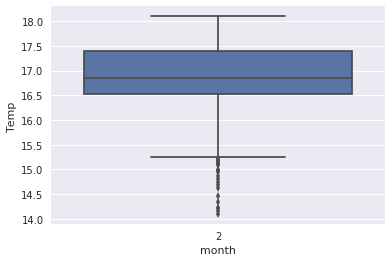
\includegraphics[width=\linewidth]{time-temp.png}
\end{figure}
\begin{figure}
\subsection{Nivel del mar y Salinidad}
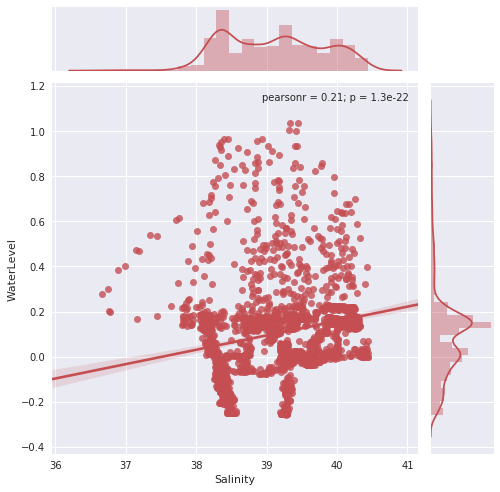
\includegraphics[width=\linewidth]{water-salinity.png}
\end{figure}
\begin{figure}
\subsection{Nivel del mar y Temperatura}
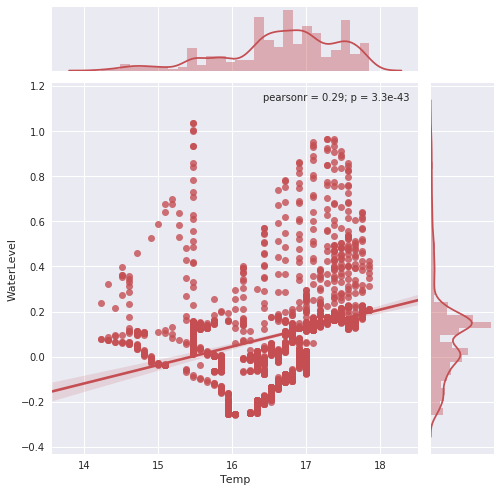
\includegraphics[width=\linewidth]{water-temp.png}
\end{figure}
\begin{figure}
\subsection{Nivel del mar y Tiempo}
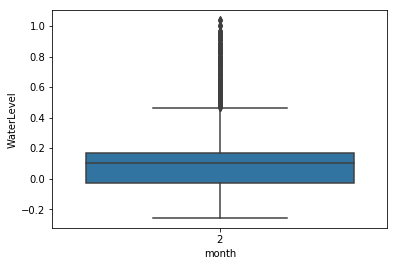
\includegraphics[width=\linewidth]{water-time.png}
\end{figure}
\end{document}
